\section*{Лекция 11 (28.04.2022)}

$\phi(t) = f(x + th)$ и хотим проверить, что $\phi^{(n)}(t) = d^n f(x + th) h ^ n$

$\phi^{(n)}(t) = \left( \frac{\partial}{\partial h} \right) ^ n f(x + th) = d^n f(x + th) h ^ n$

Следовательно любая формула Тейлора одномерная переписывается в многомерье.

\subsection{Геометрические наблюдения}

Что такое поверхность и как её задавать? (есть аналог поверхности --- многообразие, но об этом позже).

$\R ^ 3$, как задать двумерную поверхность?

Самый простой пример --- график функции.

$(x, y) \in U \text{ --- открытое } \subset \R^2$, $f : U \to \R, z = f(x, y)$

$\Gamma_f = \{ (x, y, z) \in \R ^ 3 | (x, y) \in U, z = f(x, y) \}$



% Pattern Info
 
\tikzset{
pattern size/.store in=\mcSize, 
pattern size = 5pt,
pattern thickness/.store in=\mcThickness, 
pattern thickness = 0.3pt,
pattern radius/.store in=\mcRadius, 
pattern radius = 1pt}
\makeatletter
\pgfutil@ifundefined{pgf@pattern@name@_te2ccg3cg}{
\pgfdeclarepatternformonly[\mcThickness,\mcSize]{_te2ccg3cg}
{\pgfqpoint{0pt}{0pt}}
{\pgfpoint{\mcSize+\mcThickness}{\mcSize+\mcThickness}}
{\pgfpoint{\mcSize}{\mcSize}}
{
\pgfsetcolor{\tikz@pattern@color}
\pgfsetlinewidth{\mcThickness}
\pgfpathmoveto{\pgfqpoint{0pt}{0pt}}
\pgfpathlineto{\pgfpoint{\mcSize+\mcThickness}{\mcSize+\mcThickness}}
\pgfusepath{stroke}
}}
\makeatother

% Pattern Info
 
\tikzset{
pattern size/.store in=\mcSize, 
pattern size = 5pt,
pattern thickness/.store in=\mcThickness, 
pattern thickness = 0.3pt,
pattern radius/.store in=\mcRadius, 
pattern radius = 1pt}
\makeatletter
\pgfutil@ifundefined{pgf@pattern@name@_jws2rtxgq}{
\pgfdeclarepatternformonly[\mcThickness,\mcSize]{_jws2rtxgq}
{\pgfqpoint{0pt}{-\mcThickness}}
{\pgfpoint{\mcSize}{\mcSize}}
{\pgfpoint{\mcSize}{\mcSize}}
{
\pgfsetcolor{\tikz@pattern@color}
\pgfsetlinewidth{\mcThickness}
\pgfpathmoveto{\pgfqpoint{0pt}{\mcSize}}
\pgfpathlineto{\pgfpoint{\mcSize+\mcThickness}{-\mcThickness}}
\pgfusepath{stroke}
}}
\makeatother
\tikzset{every picture/.style={line width=0.75pt}} %set default line width to 0.75pt        

\begin{tikzpicture}[x=0.75pt,y=0.75pt,yscale=-1,xscale=1]
%uncomment if require: \path (0,300); %set diagram left start at 0, and has height of 300

%Shape: Axis 2D [id:dp4017952366296539] 
\draw  (195,194.9) -- (397,194.9)(215.2,32) -- (215.2,213) (390,189.9) -- (397,194.9) -- (390,199.9) (210.2,39) -- (215.2,32) -- (220.2,39)  ;
%Straight Lines [id:da922032671850997] 
\draw    (215.2,194.9) -- (128.41,281.69) ;
\draw [shift={(127,283.1)}, rotate = 315] [color={rgb, 255:red, 0; green, 0; blue, 0 }  ][line width=0.75]    (10.93,-3.29) .. controls (6.95,-1.4) and (3.31,-0.3) .. (0,0) .. controls (3.31,0.3) and (6.95,1.4) .. (10.93,3.29)   ;
%Shape: Polygon Curved [id:ds4254674330596585] 
\draw  [pattern=_te2ccg3cg,pattern size=6pt,pattern thickness=0.75pt,pattern radius=0pt, pattern color={rgb, 255:red, 0; green, 0; blue, 0}] (259,209) .. controls (279,199) and (275,209) .. (289,232) .. controls (303,255) and (300,227) .. (320,257) .. controls (340,287) and (279,299) .. (259,269) .. controls (239,239) and (239,219) .. (259,209) -- cycle ;
%Shape: Polygon Curved [id:ds8267901841125391] 
\draw  [pattern=_jws2rtxgq,pattern size=6pt,pattern thickness=0.75pt,pattern radius=0pt, pattern color={rgb, 255:red, 0; green, 0; blue, 0}] (277,82) .. controls (288,97) and (293,82) .. (307,105) .. controls (321,128) and (369,105) .. (338,130) .. controls (307,155) and (297,172) .. (277,142) .. controls (257,112) and (266,67) .. (277,82) -- cycle ;
%Straight Lines [id:da14489689318508403] 
\draw [color={rgb, 255:red, 208; green, 2; blue, 27 }  ,draw opacity=1 ][line width=2.25]    (312,265) -- (332.39,132.95) ;
\draw [shift={(333,129)}, rotate = 98.78] [color={rgb, 255:red, 208; green, 2; blue, 27 }  ,draw opacity=1 ][line width=2.25]    (17.49,-5.26) .. controls (11.12,-2.23) and (5.29,-0.48) .. (0,0) .. controls (5.29,0.48) and (11.12,2.23) .. (17.49,5.26)   ;
%Curve Lines [id:da5494709365240873] 
\draw [color={rgb, 255:red, 65; green, 117; blue, 5 }  ,draw opacity=1 ][line width=3]    (253,243) .. controls (293,213) and (261,287) .. (301,257) ;
%Curve Lines [id:da7110344363569361] 
\draw [color={rgb, 255:red, 65; green, 117; blue, 5 }  ,draw opacity=1 ][line width=3]    (270,113) .. controls (310,83) and (278,157) .. (318,127) ;

% Text Node
\draw (338,205.4) node [anchor=north west][inner sep=0.75pt]  [color={rgb, 255:red, 208; green, 2; blue, 27 }  ,opacity=1 ]  {$f$};
% Text Node
\draw (342,263.4) node [anchor=north west][inner sep=0.75pt]    {$u$};
% Text Node
\draw (233,14.4) node [anchor=north west][inner sep=0.75pt]    {$z$};
% Text Node
\draw (110,254.4) node [anchor=north west][inner sep=0.75pt]    {$x$};
% Text Node
\draw (417,192.4) node [anchor=north west][inner sep=0.75pt]    {$y$};


\end{tikzpicture}

На поверхности можно определить систему координат --- криволинейные координаты

координаты линии --- образ множеств $x = const, y = const$

Если есть путь $\gamma[a, b] \to U $ в $U$ $\hence$ $(\gamma, f \circ \gamma)$ --- путь на поверхности.

$f$ гладкое отображение $\hence$ можно определить касательную плоскость в точке $(x_0, y_0, f(x_0, y_0))$

Двумерный аналог:\\

\tikzset{every picture/.style={line width=0.75pt}} %set default line width to 0.75pt        

\begin{tikzpicture}[x=0.75pt,y=0.75pt,yscale=-1,xscale=1]
%uncomment if require: \path (0,300); %set diagram left start at 0, and has height of 300

%Shape: Axis 2D [id:dp4017952366296539] 
\draw  (195,194.9) -- (397,194.9)(215.2,32) -- (215.2,213) (390,189.9) -- (397,194.9) -- (390,199.9) (210.2,39) -- (215.2,32) -- (220.2,39)  ;
%Curve Lines [id:da08162621152210436] 
\draw    (247,147) .. controls (287,117) and (330,164) .. (375,93) ;
%Straight Lines [id:da7039980638132205] 
\draw [color={rgb, 255:red, 208; green, 2; blue, 27 }  ,draw opacity=1 ][line width=1.5]    (395,99) -- (278,163) ;

% Text Node
\draw (233,14.4) node [anchor=north west][inner sep=0.75pt]    {$y$};
% Text Node
\draw (417,192.4) node [anchor=north west][inner sep=0.75pt]    {$x$};
% Text Node
\draw (322,202.4) node [anchor=north west][inner sep=0.75pt]    {$x_{0}$};
% Text Node
\draw (383,120.4) node [anchor=north west][inner sep=0.75pt]    {$y=f( x_{0}) +f'( x_{0})( x-x_{0})$};


\end{tikzpicture}

Тогда по аналогии уравнение аффинной касательной плоскости: $z = f(x_0, y_0) + df(x_0, y_0) \begin{pmatrix}
    x - x_0\\
    y - y_0
\end{pmatrix}$

$ = f(x_0, y_0) + \frac{\partial f}{\partial x} (x_0, y_0) (x - x_0) + \frac{\partial f}{\partial y} (x_0, y_0)(y - y_0) = $

$ = f(x_0, y_0) + \left \langle \nabla f(x_0, y_0), \begin{pmatrix}
    x - x_0 \\
    y - y_0
\end{pmatrix} \right \rangle$

А касательная плоскость сдвинута в 0 : $\left \{ (x, y, z) \, | \, z = df(x_0, y_0) \begin{pmatrix}
    x\\
    y
\end{pmatrix} \right \}$

\quad

\underline{ Касательные векторы } \\

\begin{definition}
   \begin{enumerate}
       \item элементы касательной плоскости
       \item касательные векторы к гладким путям на поверхности
    \end{enumerate}

    $(1) \Longleftrightarrow (2)$
\end{definition}

$\ola$ 

Берем $\gamma(t) = (x(t), y(t))$ путь в $U$, по нему строим путь на поверхности 

$(\gamma(t), f(\gamma(t))) = (x(t), y(t), f(x(t), y(t))) \rightarrow$ касательный вектор

$(x'(t), y'(t), \frac{\partial f}{\partial x}(x(t), y(t)) x'(t) + \frac{\partial f}{\partial y} (x(y), y(t)) y'(t) = (x'(t), y'(t), df(\cdots) \begin{pmatrix}
    x'(t)\\
    y'(t)
\end{pmatrix})$

$\ora$

$(u, v, df(x_0, y_0)\begin{pmatrix}
    u\\
    v
\end{pmatrix}) $ --- касательный вектор

Рассматриваем $\gamma(t) = (x_0 + ut, y_0 + vt)$ и все получится.

\quad

\underline{Нормаль к поверхности} = нормаль к касательной плоскости\\

$\vec{n} (x_0, y_0) = \begin{pmatrix}
    \nabla f(x_0, y_0)\\
    -1
\end{pmatrix}$, т.к. скалярное произведение с $\begin{pmatrix}
    x\\
    y\\
    \langle \nabla f , \begin{pmatrix}
        x\\
        y
    \end{pmatrix}\rangle
\end{pmatrix}$ ноль.

\quad

$Ax + By + Cz + D = 0 \hence \vec{n} = (A, B, C)^{T}$

\quad

\underline{Обобщение}

$f : x \in R^ m \to y \in \R ^ n$, $\Gamma_f = \{ (x, f(x))\} \subset \R ^ {m + n}$

Афинное касательное пространство $y = f(x_0) + df(x_0)(x - x_0)$

Касательное пространство $\{ (x, y) \, | \, y = df(x_0) x \} = T_{x_0}f = Tf(x_0)$ 

$\dim T_{x_0}f = m$

Пространство нормалей --- $(T_{x_0} f) ^ {\perp}$, вопрос, есть ли что-то лучше?

\subsection{Теорема о неявном отображении}

\begin{namedtheorem}{о сжимающем отображении}
$
        f : X \to X, X \text{ --- полное метрическое пространство}
$
\[
    \exists \gamma < 1, \forall x_1, x_2 \in X, \rho(f(x_1), f(x_2)) \leqslant \gamma \rho(x_1, x_2) \hence \exists ! x_{*} \text{ --- неподвижная точка } \in X, f(x_{*}) = x_{*}.
\]

\end{namedtheorem}


Идея: $x ^ 2 + y ^ 2 - 1 = 0$ --- не график функции. 

\quad

\tikzset{every picture/.style={line width=0.75pt}} %set default line width to 0.75pt        

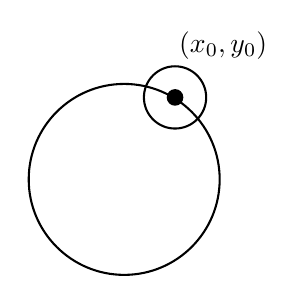
\begin{tikzpicture}[x=0.75pt,y=0.75pt,yscale=-1,xscale=1]
%uncomment if require: \path (0,300); %set diagram left start at 0, and has height of 300

%Shape: Circle [id:dp6462308613976623] 
\draw   (172,118) .. controls (172,92.59) and (192.59,72) .. (218,72) .. controls (243.41,72) and (264,92.59) .. (264,118) .. controls (264,143.41) and (243.41,164) .. (218,164) .. controls (192.59,164) and (172,143.41) .. (172,118) -- cycle ;
%Shape: Circle [id:dp584125313702382] 
\draw  [fill={rgb, 255:red, 0; green, 0; blue, 0 }  ,fill opacity=1 ] (239,78.5) .. controls (239,76.57) and (240.57,75) .. (242.5,75) .. controls (244.43,75) and (246,76.57) .. (246,78.5) .. controls (246,80.43) and (244.43,82) .. (242.5,82) .. controls (240.57,82) and (239,80.43) .. (239,78.5) -- cycle ;
%Shape: Circle [id:dp291471197461873] 
\draw   (227.5,78.5) .. controls (227.5,70.22) and (234.22,63.5) .. (242.5,63.5) .. controls (250.78,63.5) and (257.5,70.22) .. (257.5,78.5) .. controls (257.5,86.78) and (250.78,93.5) .. (242.5,93.5) .. controls (234.22,93.5) and (227.5,86.78) .. (227.5,78.5) -- cycle ;

% Text Node
\draw (243,45.4) node [anchor=north west][inner sep=0.75pt]    {$( x_{0} ,y_{0})$};


\end{tikzpicture}

В окрестности $(x_0, y_0)$ это почти наверное график фукнции.

$G(x, y) = x ^ 2 + y ^ 2 - 1$, если $\partial _y G(x_0, y_0) \neq 0 \hence $ график функции $y$ от $x$.

\[
    \underbrace{\begin{cases}
        g_1(x_1, \cdots, x_m, y_1, \cdots, y_n) = 0 \\
        \cdots\\
        g_n(x_1, \cdots, x_m, y_1, \cdots, y_n) = 0
    \end{cases}}_{G(x, y) = 0} \underset{\text{Решить систему уравнений относительно $y_1, \cdots, y_n$}}{\Longrightarrow}
    \begin{cases}
        y_1 = f_1(x_1, \cdots, x_m)\\
        \cdots\\
        y_n = f_n(x_1, \cdots, x_m)
    \end{cases} 
\]

--- график отображ. $ f : \R ^ m \to \R ^ n$

$\{ (x_1, \cdots, x_m, y_1, \cdots, y_n) | \text{ удовлетвор. сист.уравнений} \} \subset \R ^ {n + m}$

\begin{namedtheorem}{о неявном отображении}
    $X, Y, Z$ --- нормированные пространства, $Y$ --- полное

    $W \text{открытое} \subset X \times Y$, $G : W \to Z$, $(x_0, y_0) \in W$, $G$ непрерывное в $(\cdot)$ $(x_0, y_0)$, $G(x_0, y_0) = 0$,

    $\partial_y G$ существует во всех точках $W$ и непрерывен в $(\cdot) (x_0, y_0)$,

    $\exists (\partial_y G(x_0, y_0)) ^ {-1} \in L(Z, Y)$.

    $\hence \exists U$ --- окр. $(\cdot)x_0$, $V $ --- окр. $(\cdot) y_0$, $f : U \to V$ непр. в $(\cdot) x_0$

    т.ч. $\{ G(x, y) = 0 \} \cap (U \times V) = \{ (x, f(x)) \, | \, x \in U \}$
\end{namedtheorem}

\begin{proof}
    $g_x : y \in Y \to y - (\partial_y G(x_0, y_0)) ^ {-1} G(x, y) \in Y$

    Если вспомнить разговор про метод Ньютона:

    $f(x) = 0 \Rightarrow g(x) = x - \lambda f(x)$ и применить метод простых итераций.

    Посмотрим на дифференциал:

    $dg_x(y) = I_y - (\partial_y G(x_0, y_0)) ^ {-1} \underbrace{\partial_y G(x, y)}_ {\to \partial_y G(x_0, y_0), (x, y) \to (x_0, y_0) } \to 0$, при $(x, y) \to (x_0, y_0)$.

    $\exists \Delta > 0 : \max{(\norm{x - x_0} , \norm{y - y_0})} < \Delta \hence \norm{dg_x(y)} < \frac{1}{2}$

    $g_{x_0}(y_0) = y_0$, $\forall \varepsilon > 0 \exists \delta > 0 : \norm{x - x_0} < \delta \hence \norm{g_x(y_0) - g_{x_0}(y_0)} < \varepsilon$

    Хотим выбрать шарик $B$ с центром в $y_0$, т.ч. $g_x(B) \subset B$

    $\forall x : \norm{x - x_0} < \delta, \norm{x - x_0} < \Delta$

    $ g_x(\{ \norm{y - y_0} \leqslant 2 \varepsilon \}) \subset \{ \norm{y - y_0} \leqslant 2 \varepsilon \}$

    $y : \norm{y - y_0} \leqslant 2 \varepsilon$

    $\norm{g_x(y) - y_0} = \norm{g_x(y) - g_{x_0}(y_0)} \leqslant \underbrace{\norm{g_x(y) - g_x(y_0)}}_{\underbrace{\sup \norm{dg_x(\theta)}}_{\leqslant \frac{1}{2}} \cdot \underbrace{\norm{y - y_0}}_{\leqslant 2 \varepsilon}} + \underbrace{\norm{g_x(y_0) - g_{x_0}(y_0)}}_{< \varepsilon} \leqslant 2 \varepsilon$

    $g_x : B \to B$ --- сжимающее отображение $\hence \forall x\,\, \exists! \,\, y : g_x(y) = y \Longleftrightarrow G(x, y) = 0$. Тогда этот единственный $y$ и есть $f(x)$.

    $V = B_{2\varepsilon}(y_0), U = B_{\min(\delta, \Delta)}(x_0)$
\end{proof}

\begin{remark}
\quad
    \begin{enumerate}
        \item В конечномерном случае, если $\exists (\partial_y G(x_0, y_0))^ {-1} \hence $ оно обязательно из $L(Z, Y)$
        \item $\exists (\partial_y G(x_0, y_0))^{-1} \Longleftrightarrow $ обратимости матрицы. В частности $\dim Y = \dim Z$.
    \end{enumerate}
\end{remark}